\chapter{Introduction}
\label{ch:intro}

The work presented in this Theses pertains the content of the curricular internship carried out from November 2020 through December of the same year.

The curricular internship, part of the required credits for the Bachelor's Degree in Computer Science at the University of Trento, was performed remotely\footnote{%
Due to regulations related to the Coronavirus epidemic, on-premises internship have been discouraged, and should have only been performed in case of necessity. Such was not the case for the work presented here. See \cite{faq-covid} for further details.}
at SpazioDati, a technology company based in Trento, for their product Atoka.

\begin{quote}
SpazioDati works on applying Semantic Text Analysis and Machine Learning models on massive amounts of corporate data to provide services -- both B2B and B2C -- of Sales Intelligence, Lead Generation, Data Cleansing, and more.
Our main product, Atoka, is used by thousands of small and big companies in Italy and abroad. The underlying graph also powers Dandelion API, a state-of-the-art text analytics semantic engine.\footnote{%
Description via \url{https://datarade.ai/data-providers/spaziodati/profile}, last visited \today.
}

Atoka is the latest SpazioDati product which, thanks to Big Data and semantics, collects detailed information on 6 million companies in Italy and 4 million companies in the United Kingdom.
Atoka allows you to create and extract extremely precise and targeted ``customer lists'', minimizing the information asymmetry that marketing managers and sales managers often face when undertaking a business development campaign.
Atoka provides companies with all the information on potential targets, as well as for monitoring the evolution of the market and competitors.
In other words, it facilitates B2B lead generation and allows access to a daily updated database of 6 million Italian companies and 4 million British companies, thanks to the partnership with Cerved Group.
No other provider in Italy is able to support such numbers, the accuracy and freshness of the data are critical success factors: with 500 million web pages and 70 thousand news items analyzed, Atoka allows Sales and Marketing Intelligence actions never seen before in the Italian market.\footnote{%
Ibid.
}
\end{quote}


\section{Non Disclosure}
\label{sec:non-disclosure}

In this document several information internal to SpazioDati is referenced.
In order to avoid disclosing information relevant to their intellectual property, the relational tables later referenced in this Theses have been anonymized.

In particular the names of the eleven tables referenced have been replaced with the Greek letters $\alpha$, $\beta$, $\gamma$, $\delta$, $\epsilon$, $\zeta$, $\eta$, $\theta$, $\iota$, $\kappa$, and $\lambda$.
Additionally, referenced column names do not represent the real names used in SpazioDati; nevertheless they provide a sensible metaphor to their actual counterpart. 

TODO
The contents of this Theses have been reviewed by SpazioDati and they have acknowledged this document does not contain information sensitive to either their customers or their intellectual properties.


\section{Problem Statement}
\label{sec:problem-statement}

Before stating the matter at hand, let us first consider the prior rationale for this endeavor.

Since the Atoka service has a subscription-based business model,\footnote{%
I.e. users pay a recurring fee for access to the service and may decide to stop paying (discontinuing the subscription), according to the terms of service.
} one important problem considered by the marketing team is the necessity to keep already-subscribing users engaged with the product, so as to induce a continuation of the subscription.

The marketing team has considered that a user, presented with insightful data about his usage of the product, would observe his possible under-usage, or learn techniques to a more efficient usage of Atoka.
%Additionally, the marketing team would acquire an instrument to better understand how their customers utilize the product.

This would be achieved by investigating said usage of the product, employing activities data recorded on their internal relational database services.

Since the queries intended for this application are computationally expensive, instead of running those queries directly on the main database, it was decided the database would emit data change events\footnote{%
Here, \emph{data change events} refers to a series of events that can be used to reproduce the changes that have occurred in the database.
The actual meaning of this expression will become clearer in \S \ref{sec:cdc}.
} that would be sent to, and recorded in, a separate database, used specifically for this application.

By design, such a mechanism effectively produces data duplication, but impacting the performance of Atoka's database service (thus degrading the overall user experience) was valued a problem much greater than the expense of data replication.

The queries carried out by the marketing team are, though, of little concern for this Theses.
Our interest lies in making the data involved available to the team, which will later employ it as they deem fit.


\section{Change Data Capture Systems}
\label{sec:cdc}

In the previous Section, the necessity to record data as it was modified emerged.
Such need may be fulfilled by a Change Data Capture (CDC) system;\footnote{%
For further reference see \cite{cdc}.
} in this Section we will go over what it amounts to.

With \emph{change data} we refer to data regarding a modification of some data source's contents; thus, logically, CDC systems are composed of at least a data source.\footnote{%
Which may also be a component of other systems.}
Along with it, a CDC system requires a mechanism to deliver this data to some sub-systems that consume it.
As such, we can outline at least three different components of a CDC system: a data source, a change data broker, and one or several consumer sub-systems.

The broker is intended as a delivery mechanism for messages, by which we mean content (i.e. in our case, change data) interchanged between systems.
What we expect from this sub-system is that messages are delivered to consumers in the order they were received, are consumed exactly once, and have negligible delay.

In Figure \ref{fig:cdc-generic} a generic outline of a CDC system is presented.

Furthermore, in the case at hand, a PostgreSQL server is the data source, Apache Kafka (along with Kafka Connect, and a Debezium Connector) is the broker, and the several consumers are Kafka Connect Sinks, additionally enriched with Kafka Streams.\footnote{Cf. Chapter \ref{ch:techs}.}
In Figure \ref{fig:cdc-complete} the overall system, i.e. the content of this Theses, is presented; relations to parts of a generic CDC system are outlined with dashes.

As previously mentioned, the presented CDC system's output is stored in a PostgreSQL database, which has been specifically created for the purpose discussed in \S \ref{sec:problem-statement}.
It must not be confused with the data source.

\begin{figure}
\centering
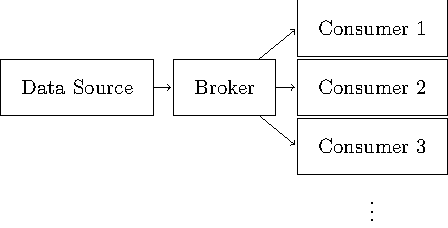
\includegraphics[]{figures/introduction/cdc-generic}
\caption{A Generic CDC System.}
\label{fig:cdc-generic}
\end{figure}

\begin{figure}
\centering
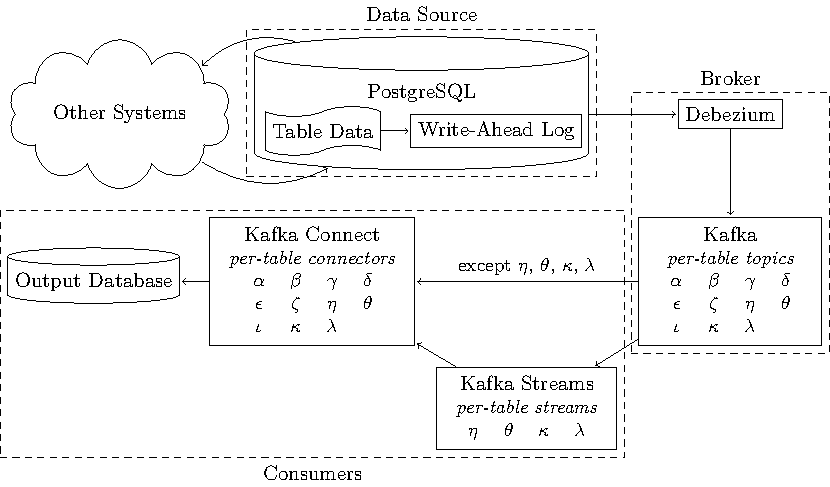
\includegraphics[width=\linewidth]{figures/introduction/cdc-complete}
\caption{An Outline of the CDC System presented in this Theses.}
\label{fig:cdc-complete}
\end{figure}



\section{On the Duality between Tables and Streams}
\label{sec:tables-streams}

We have since said that there would be a relational database as data source, another one as the output of the CDC system, and in between we have talked about some \emph{events}.
Clearly, as these events are materialized as messages, they do not pertain to a relational data model; instead they refer to a streaming data model, in which several messages are interchanged.
Spontaneously, a question arises: how do these two models coexist and sustain a back and forth translation?

The answer is to be found in the two fundamental concepts of the models.
%In this Section, I will sustain the following claim: 
%\begin{quote}
%A table can be interpreted as a stream; and a stream can be interpreted as a table.
%\end{quote}

Let us consider a table (or relation) $T$.
If this table is updated (i.e. a row is inserted, deleted or changed) we say there is a change data event $\delta$.
We can define an ordered unbounded sequence $\Delta$ of all changes to $T$, which is the stream of changes to $T$.

Let us define a sum of changes as the sequential application of data change events to some relation, such that $\delta + \epsilon$ is some data change, defined as the sequential application of $\delta$ and then $\epsilon$, for any $\delta$ and $\epsilon$ being two sequential data change events in $\Delta$.
Let us consider $\alpha$ as the sum of all changes in $\Delta$:
$$
\alpha = \sum_{\delta \in \Delta} \delta \; .
$$
It is trivial to assert that $ \alpha = T $, which is to say that a table may be re-composed from the sequential application of its data change events.

Considering all of the above, we can conclude that the streaming of data change events of any table $ T $ is an alternative representation of $ T $.


\section{Notation}

In the following chapters we'll make use of standard notation for Relational Algebra, best described in \cite[Chapter 4]{dbms}.

Additionally, further notation will be introduced in order to allow for clarity between table representations, and formal discussion of aggregation queries.


\subsection{Source and Destination Tables}

Every table has one representation in the source database and another representation in the destination database.
Thus simply referring to some table $\omega$ may be ambiguous, given the identical names of the two representations.

To avoid such ambiguity, let us introduce the following notation:

\begin{itemize}
	\item $\source{\omega}$ and $\dest{\omega}$ refer to the representation of some table $\omega$ at the source and destination databases respectively;
	\item $\source{*}$ and $\dest{*}$ refer to the representations of all tables collectively (i.e. the whole databases), at the source and destination databases respectively.
\end{itemize}

It should be noted that the source tables are spread between different logical, as well as physical locations; i.e. different relational databases, not hosted on the same server.
This, though, should be of little interest: as better explained in the following chapters, the different source tables are represented into as many topics on the same Kafka cluster (cf. \S \ref{sec:kafka}), abstracting away from the source.
Therefore, $\source{\omega}$ refers to the source representation of table $\omega$, regardless of where, even logically, it is stored.


\subsection{Aggregation Related Functions}

Common constructs of Relational Algebra do not provide a way in which one can express aggregation queries.\footnote{%
See remark in \cite[p.~154]{dbms}.
}

Effectively, this renders the notation defined in this section into something that is not Relational Algebra, since it does not satisfy the closure property, as shown later.
Nonetheless, I argue that there can be a strict separation between relational algebra and the notation that will shortly be introduced.
Also, a well-defined way for going back and forth between these different notations will be laid down.

\begin{definition}[Grouping generation]\label{def:G}
Let $G$ be the grouping generation operator, $\omega$ any relation, and $c$, the grouping key, a column of $\omega$.
Let $V$ be the set of all the values of the grouping key in $\omega$.
The grouping $G_c(\omega)$ is defined as the set of relations (groups) obtained performing all the possible selections from $V$:
$$
G_c(\omega) = \{
    g : g = \sigma_{c = v}(\omega), \forall v \in V
\} \; .
$$
\end{definition}

\begin{example}\label{eg:grouping}
Let $\omega$ be the relation shown in Table \ref{tab:eg-grouping}.a.
$G_m(\omega)$ is shown in Table \ref{tab:eg-grouping}.b.

\begin{table}
\begin{center}
(a)
\begin{tabular}{ll}
\emph{m} & \emph{n} \\
\hline
a & 1 \\
b & 5 \\
a & 3 \\
\end{tabular}
\hspace{1cm}
(b)
\begin{tabular}{ll}
\emph{m} & \emph{n} \\
\hline
a & 1 \\
a & 3 \\
\end{tabular}
\begin{tabular}{ll}
\emph{m} & \emph{n} \\
\hline
b & 5
\end{tabular}
\hspace{1cm}
(c)
\begin{tabular}{ll}
\emph{m} & \emph{n} \\
\hline
a & 4
\end{tabular}
\begin{tabular}{ll}
\emph{m} & \emph{n} \\
\hline
b & 5
\end{tabular}

(d)
\begin{tabular}{ll}
\emph{m} & \emph{n} \\
\hline
a & 4\\
b & 5
\end{tabular}
\end{center}
\caption{Relations of Examples \ref{eg:grouping}, \ref{eg:grouping-selection}, and \ref{eg:grouping-merge}.}
\label{tab:eg-grouping}
\end{table}
\end{example}

\begin{observation}\label{obs:G-not-in-R}
If $\mathcal{R}$ is the set of all relations, it is evident from the above definition that $G_c(\omega) \not\in \mathcal{R}$ for any $c$ and $\omega$.
Thus, the output of the grouping generation operator is \emph{not} a relation.

Since every construct of Relational Algebra satisfies the closure property with respect to $\mathcal{R}$, the $G$ operator from Definition (\ref{def:G}) cannot be considered part of Relational Algebra.
\end{observation}

\begin{definition}[Grouping with multiple keys]
Let $C$ be a set of grouping keys, and $\omega$ any relation.
$G_C(\omega)$ is defined as
$$
G_C(\omega) = \bigcup_{c \in C}G_c(\omega) \; .
$$
\end{definition}

\begin{observation}
A grouping with multiple keys, is still a grouping (i.e. a set of relations).
\end{observation}

\begin{definition}[Grouping selection]
Let $H$ be a grouping, $C$ the set of grouping keys of $H$, \emph{f}, and \emph{h} two aggregation functions\footnote{%
Here ``aggregation functions'' is used to indicate some functions that produce a result from a succession. E.g. $\sum$, $\min$, and so on.
}, and $c_i$, and $c_j$ two columns of any group in $H$.
The grouping selection operation $\sigma^*$ is defined as the grouping
$$
\sigma^*_{f(c_i), h(c_j), \dots}(H) = \Big\{
    \big\{ \langle c : c \in C, f(g.c_i), h(g.c_j), \dots \rangle \big\} : g \in H
\Big\} \; .
$$
\end{definition}

\begin{example}\label{eg:grouping-selection}
Continuing from Example \ref{eg:grouping}, let us consider $\sigma^*_{\sum{n}}(G_m(\omega))$, as shown in Table \ref{tab:eg-grouping}.c.
\end{example}

\begin{observation}
The output of the grouping selection function $\sigma^*$ is a grouping.
Each one of the groups is a single instance relation.
\end{observation}

\begin{definition}[Grouping merge]
Let $H$ be a grouping. The merging operation is defined as
$$
M(H) = \bigcup_{g \in H} g \; .
$$
\end{definition}

\begin{example}\label{eg:grouping-merge}
Continuing from Example \ref{eg:grouping-selection}, let us now consider $M\Big(\sigma^*_{\sum{n}}(G_m(\omega))\Big)$, as shown in Table \ref{tab:eg-grouping}.d.
\end{example}

\begin{proposition}
A merged grouping is a relation.
\end{proposition}
\begin{proof}
Notwithstanding Observation (\ref{obs:G-not-in-R}); from Definition (\ref{def:G}): $\forall g \in G_c(\omega), g \in \mathcal{R}$, since it is defined as a selection.

A union of relations is a common operation of Relational Algebra, thus the result of $M(H) \in \mathcal{R}$, for any grouping $H$. 
\end{proof}
